% Chapter 5 from the standard thesis template
%   with a full page figure and a sideways table.

%Chapter 5 discusses the Experimental setup and experiments used and how I evaluated the performance of the radiometer.

\chapter{EVALUATION SETUP AND EXPERIMENTAL DESIGN}\label{ch:exp_design}
The experiments outlined in this chapter is to demonstrate and verify that a software defined radiometer is able to perform as well or better than a traditional radiometer.  In addition, it will be demonstrated that a software defined radiometer can add additional functionality not typically found in most radiometers. 

Experiment one verifies the operation of a software defined radiometer by comparing typical operations to a square-law detector, a typical device used in radiometry and calibration of the radiometer.  Experiment two verifies the expected sensitivity and stability of a software defined radiometer.  Experiment three will demonstrate a software defined radiometer mitigating an interfering signal and compare the results to a traditional radiometer with no interfering signal mitigation.  Finally, Experiment four will examine the affect filtering and bandwidth of the signal affects performance.  

\section{Experiment I - Software Defined Radiometer Verification and Calibration}\label{Exp1}
%Experiment 1
%Why is this experiment being run?
%What type of data will you collect?
%What is the experimental setup?

In this experiment we will verify the operation of a software defined radiometer.  This experiment will verify that a software defined radiometer is able to perform as expected and will compare our results to a square-law detector which is commonly used in traditional radiometers.  
To verify the results of the information that the software defined radio is obtaining a square-law detector is used to measure the power of the incoming signal in parallel to the software defined radio.  This signal is split using a power divider so that the information will be the same to both devices with the except for the 3 dB plus insertion loss the power divider adds.  This allows us to verify the software defined radio with a proven system.  

\subsection{Data Collection}\label{exp1_data}

Two sets of data is produced with this experiment.  First, data is generated from the software defined radio using GNURadio.  Second, data is generated from a data acquisitions device that is attached to the square-law detector.  Data from each one is stored to a local computer running the appropriate software.

\emph{Software Defined Radio Data.  }The data from the software defined radio is stored in files generated from GNURadio.  GNURadio uses a sink block to output the data to either a screen, socket connection such as TCP/IP or a file.  In our case we will use a file sink to output the data to a file.  The flow of data to this sink is controlled by a valve block.  This allows for the user to turn on and off recording of the data.  A block diagram of the file blocks is in figure \ref{filesink}.

{\begin{figure}[h!tb] \centering
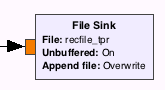
\includegraphics[width=\textwidth]{Images/TPR_Filesink.png}
\isucaption{The File Sink block used in GNURadio.  Source:  GNURadio}
\label{filesink}
\end{figure}
}

There are two types of files that the SDR generates.  The first type of file is the complete I and Q data points recorded from the SDR.  This file is stored as a little-indian format and as complex values.  Due to the sampling rate, it is not uncommon for this file to grow to be quite large, usually several gigabytes of data for a 10-15 minute run.  However, this file can then be feed back through GNURadio later to be played back if needed and it contains the information needed to completely recreate the signal.

The second file type is the total power values generated from the total power block in GNURadio.  A block diagram of this block can be found in Appendix \ref{appendix1} in figure \ref{TPR_GRC} and the source code for this can also be found in Appendix \ref{appendix1}.  This file is also a little-endian format however this file only has float values.  This file is also much smaller than the file that contains the I and Q data points.  A typical file size is 50 - 100 kB for a 10 to 15 minute run.  

\emph{Square-law detector data.}  The square-law detector outputs information as an analog voltage that is linearly proportional to the RF power measured.  This required a system that can capture the analog signal from the ADL5902 and then send the data to be stored.  The National Instruments USB-6009 data acquisition unit was selected as it met the requirements for an easy to use yet high enough resolution to obtain accurate information.  The USB-6009 unit has 8 analog inputs that can sample up to 48 ksps with a resolution of 14-bits which is more than adequate for the experiments.  To use the USB-6009 a fairly simple Lab View program was created to obtain, display and store the data from the ADL5902.  This program retrieved the information from the USB-6009 and stored the data in both Labview's binary format and in a more human friendly ASCII format.  The USB-6009 then connects to a host computer through the USB interface.  This made obtaining the data and using device straightforward to use.

The Labview program created generates a user interface to display the data and allow for turning on and off the recording.  This allowed for easy monitoring of the square-law data while the experiment was being run.  A screen shot of the GUI created in Labview is shown in figure \ref{labviewgui}.

{\begin{figure}[h!tb] \centering
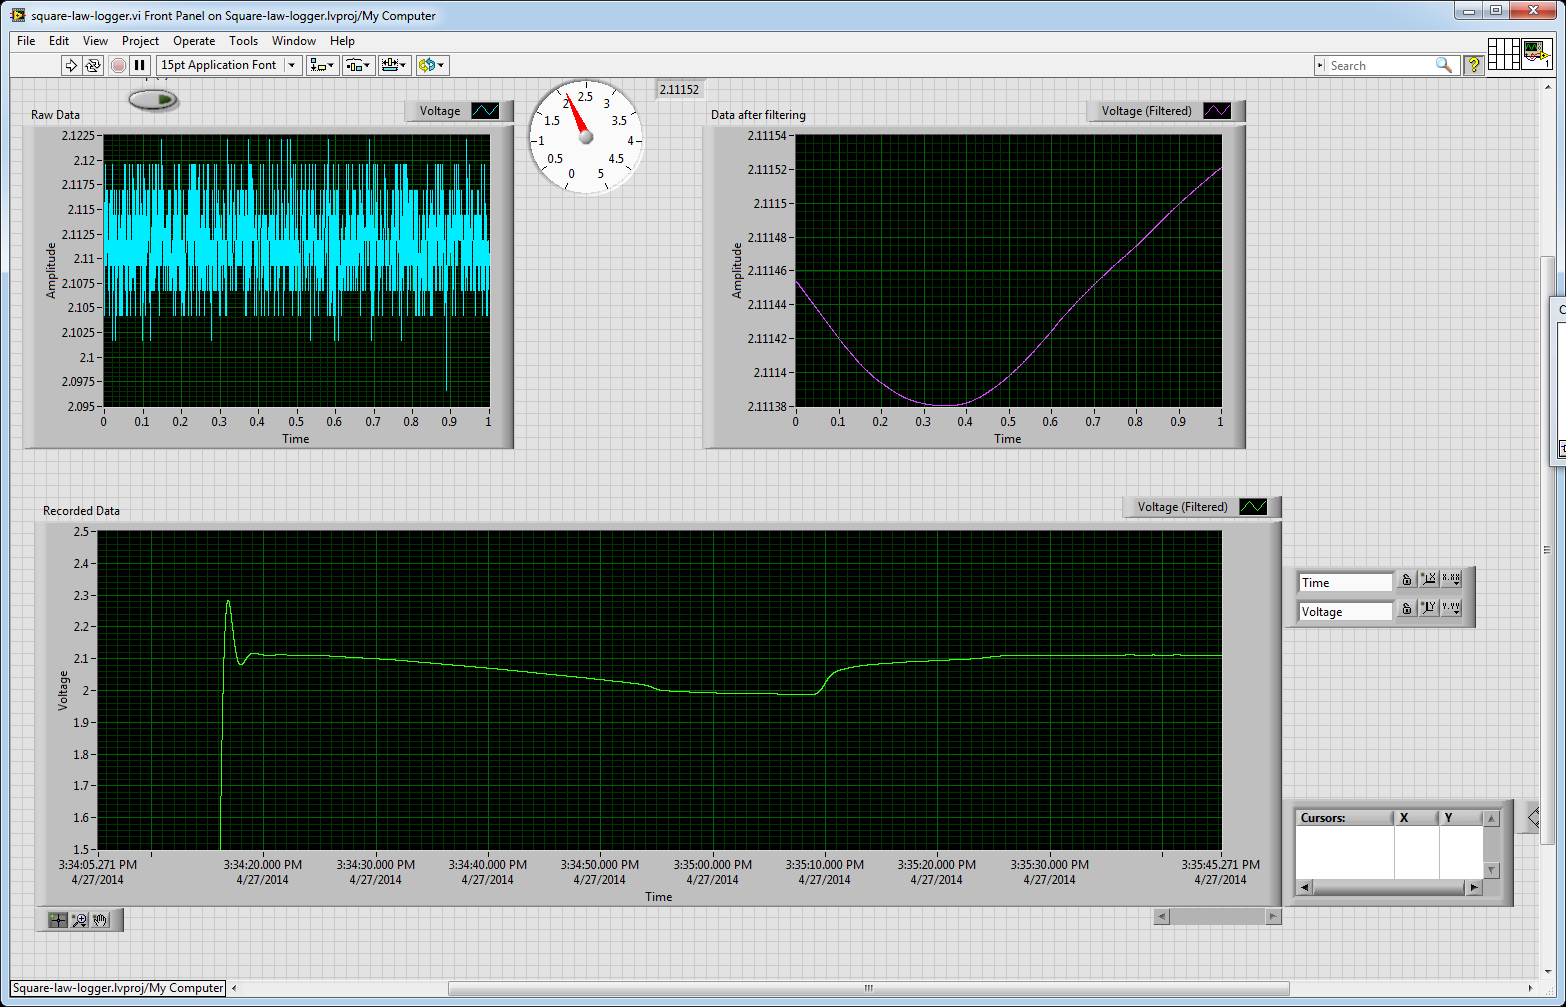
\includegraphics[width=\textwidth]{Images/labviewGUI.png}
\isucaption{A screenshot of the Labview GUI interface.  Source:  Labview}
\label{labviewgui}
\end{figure}
}

This program uses the National Instruments DAQ assistant which allows for quick configuration and setup for the computer to talk to a number of NI devices.  Labview also includes blocks that allows us to easily record the data to a file and also use a low pass filter.  These blocks made up most of the program and resulted in a program that was quickly made.  Figure \ref{labviewblock} shows the blocks used and the wiring of the blocks.

{\begin{figure}[h!tb] \centering
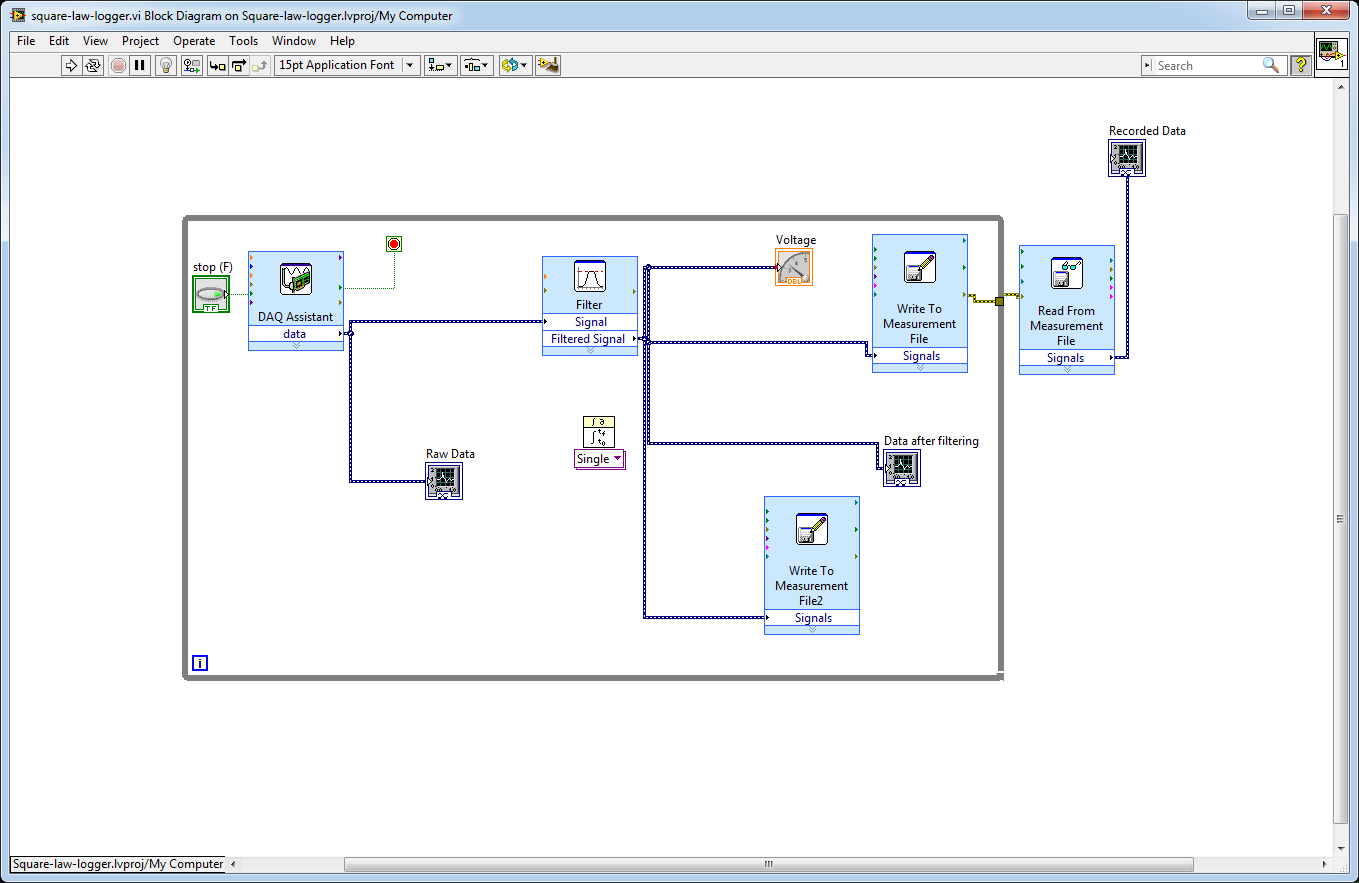
\includegraphics[width=\textwidth]{Images/labview-diagram.png}
\isucaption{A screenshot of the Labview block diagram.  Source:  Labview}
\label{labviewblock}
\end{figure}
}

\emph{GNURadio Testing.  }Before testing the program with the N200, testing was done with the built in noise generator in GNURadio.  This was used to test its ability to measure small changes in noise.  This simulated noise verified that the program written was able to detect changes in noise power using a simulated Gaussian source.  It was also desired to also use a hardware based noise generator, however a suitable noise generator could not be located on campus.

{\begin{figure}[h!tb] \centering
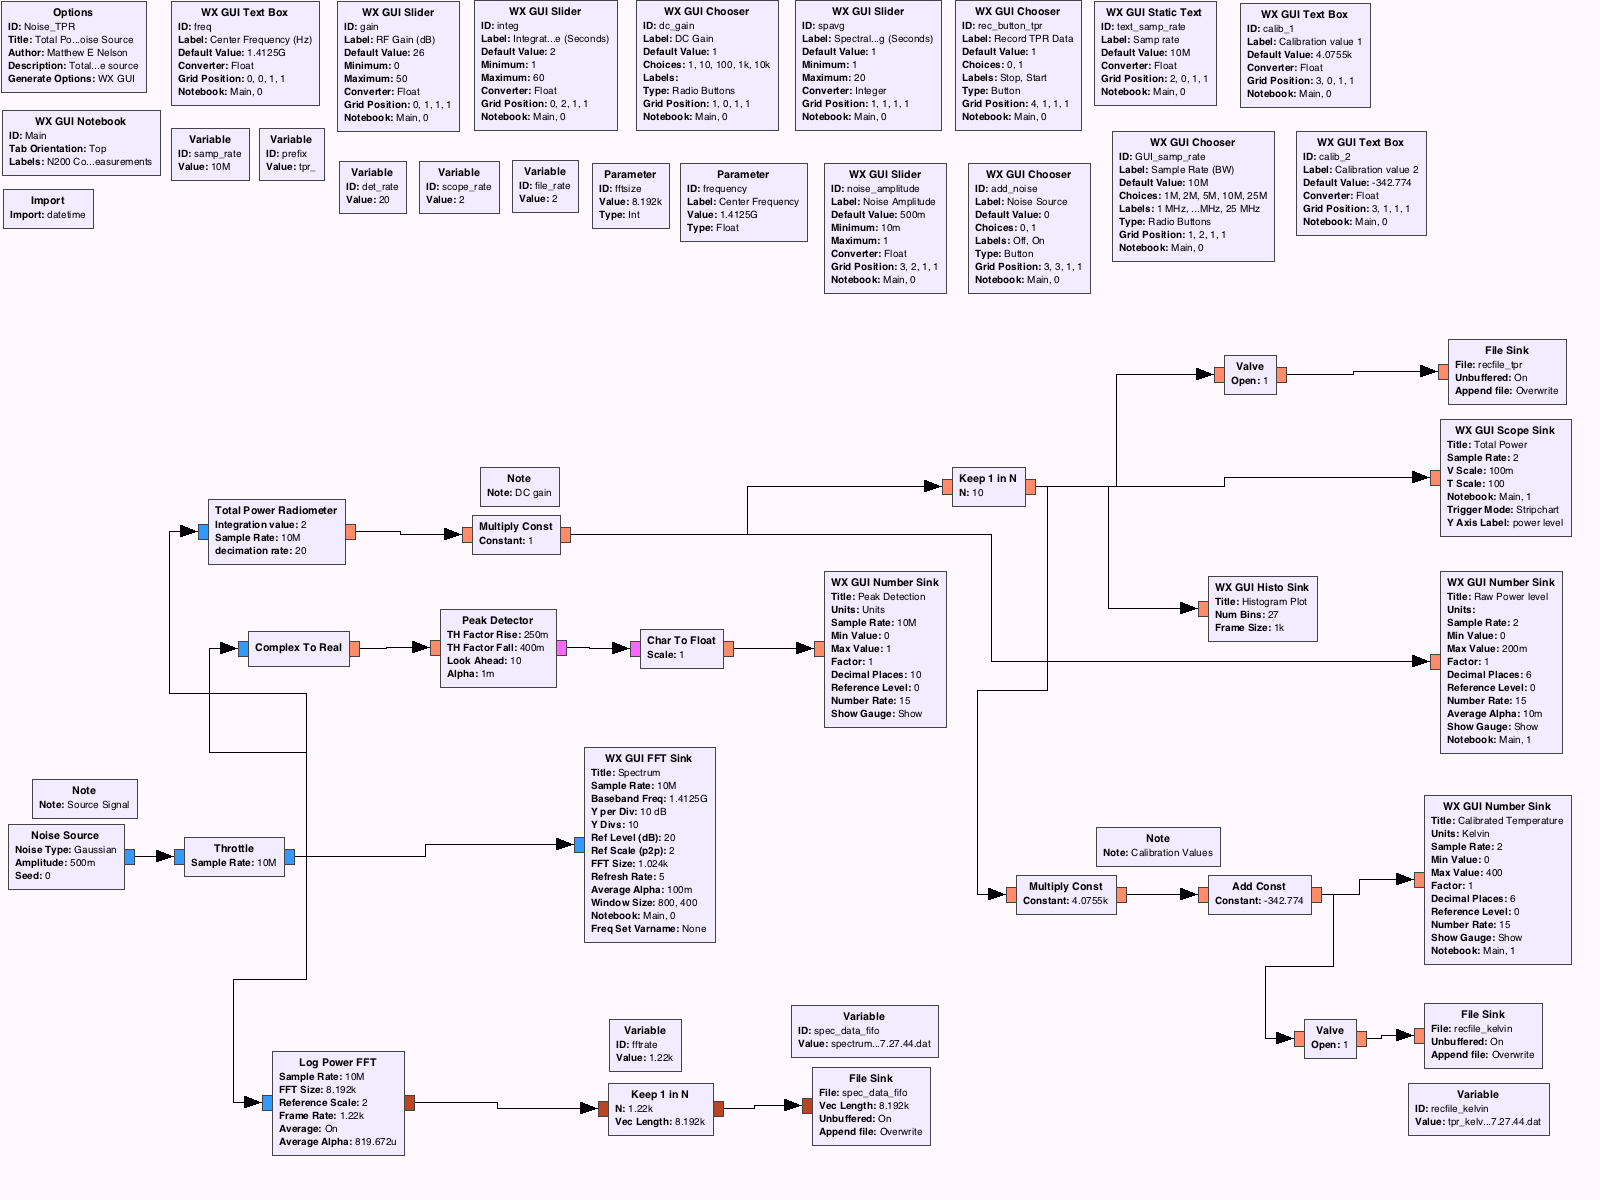
\includegraphics[width=\textwidth]{Images/noisesrc_radiometer.png}
\isucaption{A screenshot of the GNURadio program using a noise generator block.  Source:  GNURadio}
\label{noise_test}
\end{figure}
}

After this was done additional tweaks were made to both the GUI interface and to the program that performs the calculations for the total power radiometer.  The essential components were moved to a custom block which helped to clean up the block diagram.  

\subsection{Experimental setup} \label{exp1_setup}
For this experiment, the following hardware was used:

\begin{enumerate}
\item N200 Software Defined Radio with DBSRX2 Daughter-board
\item ADL5902 Square-law detector
\item National Instruments USB-6009 Data Acquisition Unit
\item ZN2PD-20-S+ Power Divider
\item 50-ohm matched load
\item Rigol DP832 Power Supply
\item ISU Radiometer RF Front End
\end{enumerate}

The ISU Radiometer, as shown in figure \ref{ISURF} was used as it has the necessary Low Noise Amplifiers (LNAs) to provide the needed amplification.  The only item powered for these experiments was the LNAs, all other components are passive or were deactivated.  The ISU Radiometer uses the following hardware:

\begin{enumerate}
\item 4 x Integrated Microwave Bandpass filters (1400 - 1425 MHz)
\item 2 x Miteq AMF-3F-01400147-30-10P LNA
\item 1 x Miteq AMF-2F-01400147-04-10P LNA
\end{enumerate}

{\begin{figure}[h!tb] \centering
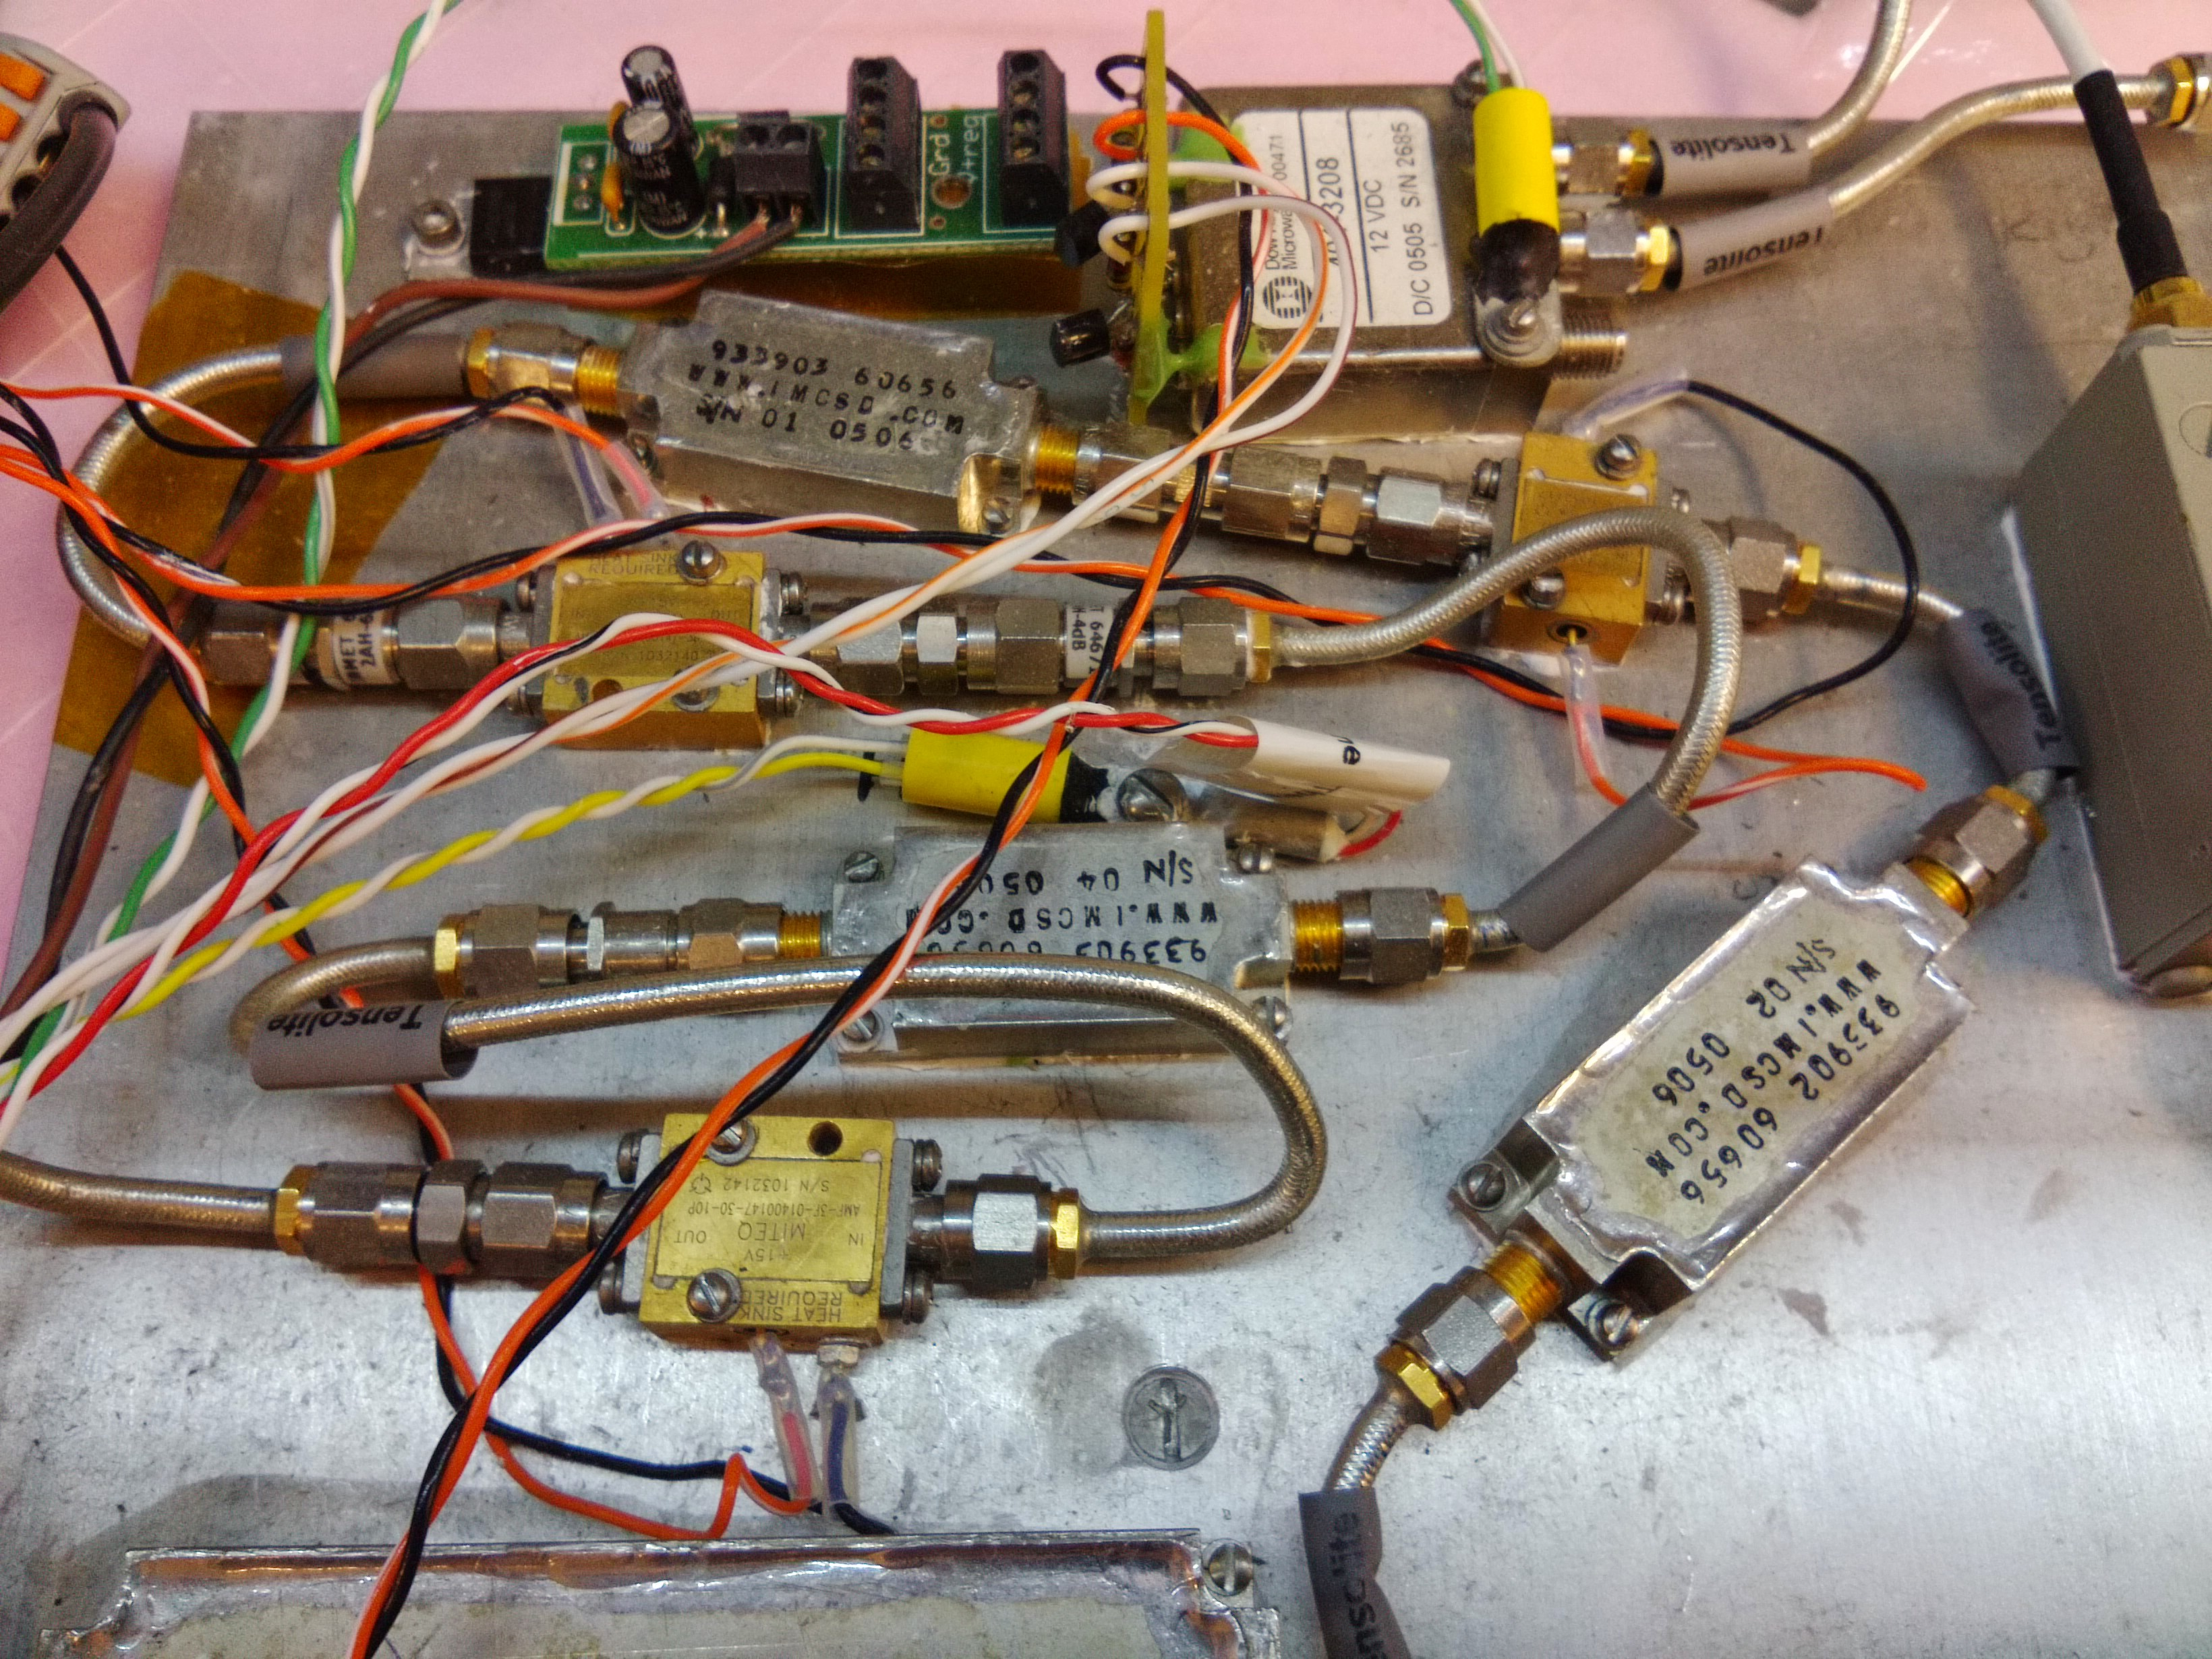
\includegraphics[width=\textwidth]{Images/ISU_RF.jpg}
\isucaption{The ISU radiometer's LNAs and bandpass filters used in most experiments.  Source: Matthew E. Nelson}
\label{ISURF}
\end{figure}
}

Figure \ref{Exp1_Block} shows a block diagram of the experimental setup.  A matched load is used to simulate our antenna or source.  This matched load is then submerged in temperature baths.  The physical temperature of this matched load is then the noise temperature the radiometer sees and can be used to calibrate the radiometer.  The ISU radiometer provides the amplification needed for our experiments and finally we divide that signal between the ADL5902 square-law detector and the N200 Software defined radio.  The N200 is then connected to a personal computer running XUbuntu Linux and GNURadio.

{\begin{figure}[h!tb] \centering
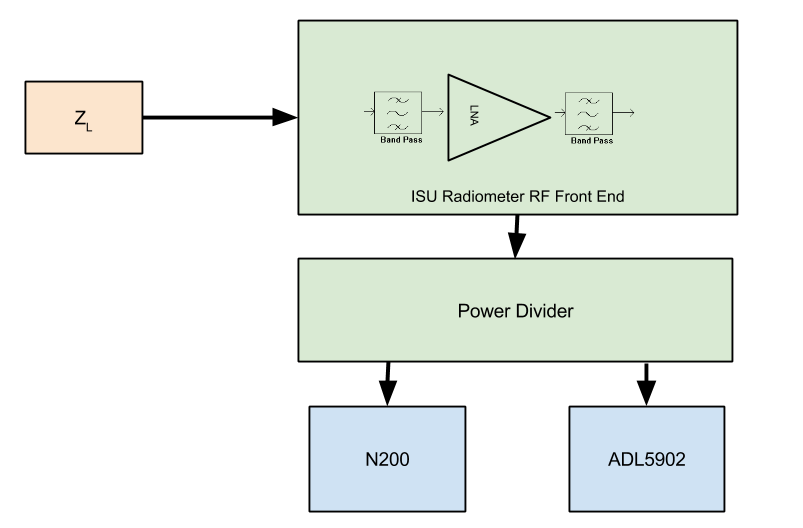
\includegraphics[width=\textwidth]{Images/Exp_1_Setup.png}
\isucaption{Block diagram of Experiment 1 setup.  Source: Matthew E. Nelson}
\label{Exp1_Block}
\end{figure}
}

The 50 ohm load was then submersed into a hot or cold bath.  These baths were temperature controlled first by using Liquid Nitrogen (LN2) which is known to boil at 77 Kelvin and an ice water bath which is known to be at 273.15 Kelvin.  The temperature of these could easily be monitored and maintained.  The load was submersed in each bath for a minimum of 2 minutes to allow for it to reach the same temperature as the bath.  The noise temperature measured was then recorded using the setup described.

%\subsection{Laboratory Setup}
%For this experiment the ISU radiometer was setup in the Make to Innovate lab located in Howe Hall at Iowa State University.  This lab was picked as it has an electronics area and has test equipment needed for certain experiments as well as the needed power supplies to power the equipment.  To measure the change in noise, a 50 ohm matched load was attached to the input of the LNAs and this output was then feed to a power divider which divides the signal between the software defined radio and the square-law detector.  This does add a 3.1 dB loss to both devices, however this was acceptable for these experiments.

%\begin{figure}[h!tb] \centering
%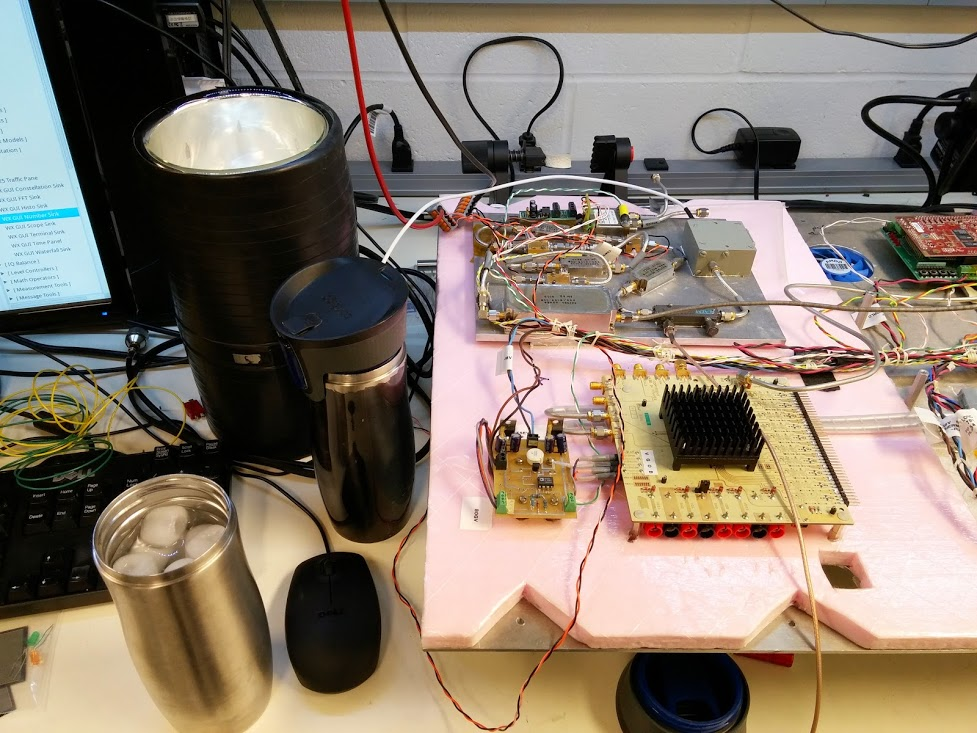
\includegraphics[width=\textwidth]{Images/exp1_setup.jpg}
%\isucaption{An image of the typical lab setup used to test the software defined radiometer}
%\label{LabSetup}
%\end{figure}

\section{Experiment II - Verification of sensitivity and stability}\label{Exp2}

In this experiment we will verify the sensitivity and stability of a software defined radiometer.  This experiment will verify that a software defined radiometer is able to meet the expected sensitivity and stability within an acceptable range.    

\subsection{Data Collection}
The data collected for this experiment was the total power measurements made from the software defined radiometer.  These measurements uses the same method as outlined in section \ref{exp1_data}.

\subsection{Experimental setup} \label{exp2_setup}


\section{Experiment III - Interfering Signal Mitigation}\label{Exp3}

In this experiment we will generate an interfering signal and then mitigate the signal using a software defined filter.  A square-law detector will be hooked up in parallel to measure the same signal but will have no mitigation methods for the signal.  We will then compare the two signals to verify that the software defined radiometer can mitigate an interfering signal and still make total power measurements.

The addition of an unwanted signal can be a determinant to the radiometer and has an adverse effect on how the radiometer operates.  In today's world though, it is getting more difficult to control intentional radiators as the RF spectrum becomes crowded with more devices.  This problem becomes even a greater issue with radiometers used in orbiting spacecrafts as they are able to see large areas[\cite{DeRooRFI}].  Even though the band we are working in of 1.4 GHz is an internationally protected frequency, there can still be both intentional and unintentional radiators that cause interference.

RFI detection and mitigation is not a new topic in radiometry and there have been other methods in both the detection and mitigation of these signals[\cite{Forte}][\cite{McIntyre_RFI}][\cite{DeRoo}][\cite{Ellingson}].

This test was designed to test a problem that a software defined radio would be to cope with while a square law detector would not be able to cope with it.  This test injected a known signal at 1.406 GHz to interfere with the normal operation of the radiometer.  In this test, the square law detector, since it is a wide band device, would not be able to accurately measure the change in the total power of the signal.  However, the SDR is able to create a digital filter to filter out the offending signal.  Since this is done in software, the SDR is able to adapt to change much faster than an analog radiometer.

Our Software Defined Radio software is now altered to include a band-reject filter that will filter out the offending signal.  The filter was first designed using the included GNU Radio Filter Design tool that is part of the suite of software with GNURadio.  Figure \ref{GRC_Filter_DSN} shows a screen shot of the tool when designing the band-reject filter for this application.  This tool generates filter values also called taps that GNURadio will use for defining the filter.  The GUI program shown in figure \ref{GRC_Filter_DSN} allows us to interactively create a filter.  However, in our GNURadio program, we can call this program directly from our program to generate the taps needed.  This is quite easy to do since both GNURadio and the program that generates the taps are both Python programs.  

\begin{figure}[h!tb] \centering

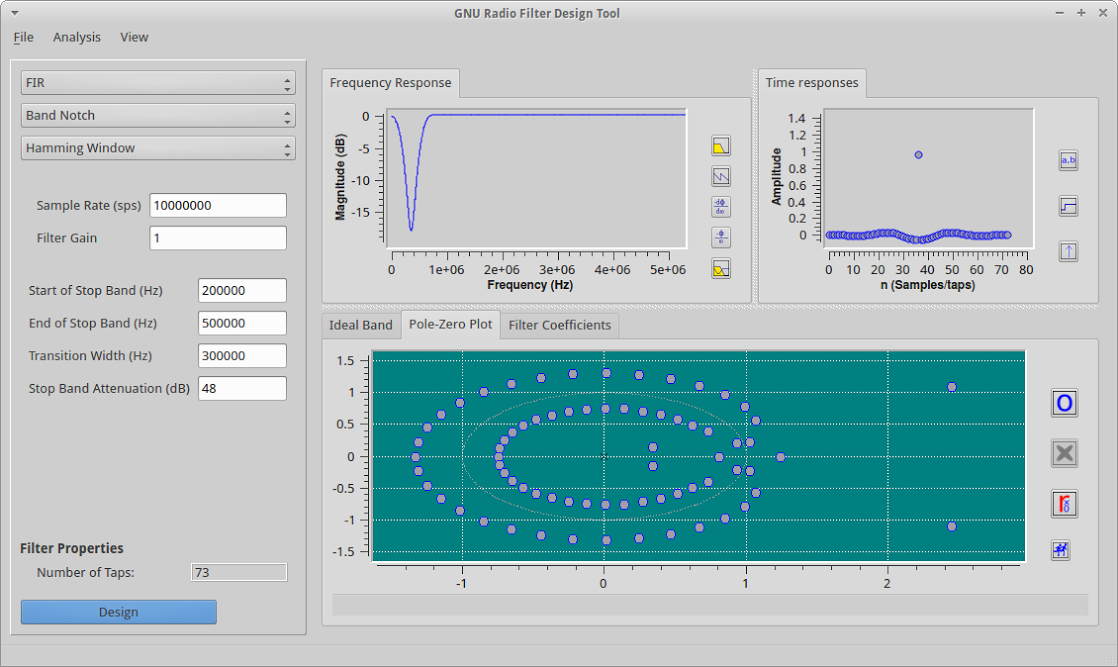
\includegraphics[width=\textwidth]{Images/GNURadio_Filter_dsn.png}
\isucaption{Image of the GNU Radio Filter Design tool}
\label{GRC_Filter_DSN}
\end{figure}  

Now that the taps have been calculated it is now applied to the filter in the system.  The band-reject filter will of course affect our performance as we will lose some bandwidth to the filter.  However, as shown it is still possible to function as a total power radiometer while filtering this signal.  

\subsection{Data Collection}

The data collected for this experiment includes both the total power measurements and the square-law data.  Section \ref{exp1_data} explains in detail the setup and configuration of the equipment used to collect this data.

\subsection{Experimental setup} \label{exp3_setup}

The experimental setup for this experiment is similar to the setup outline in section \ref{Exp1}.  In addition to the setup outline in that section, another software defined radio was added and injected into the RF signal chain.  This software defined radio is then configured to operate like a signal generator and generates the offending signal.  

Our signal generator is the HackRF One shown in figure \ref{HackRF}.  This SDR is a cheaper SDR and thus has lower specifications than the Ettus Research N200 used as the software defined radiometer.  However, for the task of a signal source, it will suit our needs.

\begin{figure}[h!tb] \centering

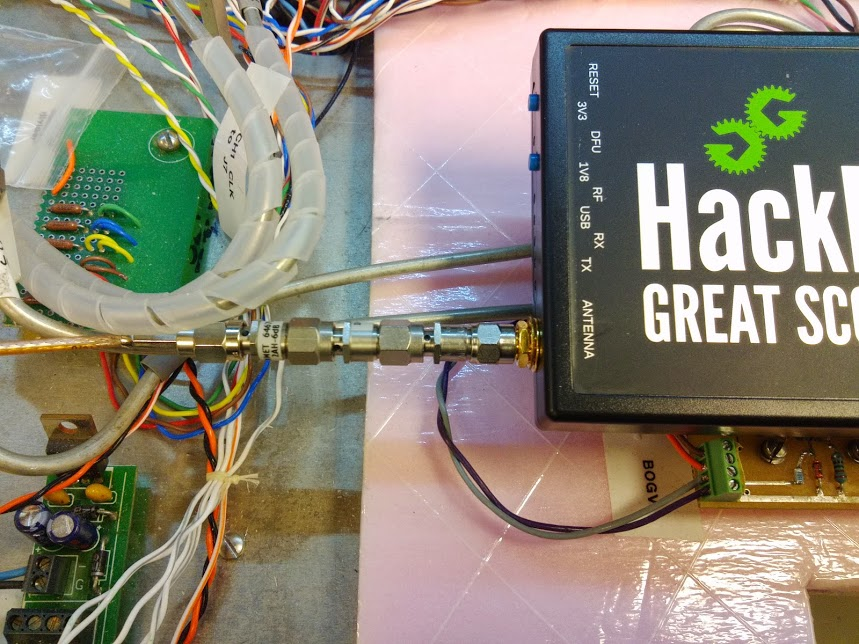
\includegraphics[width=\textwidth]{Images/Hack_RF.jpg}
\isucaption{Image of the HackRF used to generate the offending signal}
\label{HackRF}
\end{figure} 

For this experiment, the HackRF will generate a sinusoidal wave at a fixed frequency.  We will then change the amplitude of this signal a few times during the experiment.  This allows us to verify that the signal is still present in the total power measurements in both the software defined radio and the square-law detector.  Since the square-law detector does retain any frequency information, this was the only method to verify the operation of the signal generator with the square-law detector.   

\section{Experiment 4 - Performance impact of interfering signal mitigation}\label{Exp4}

\subsection{Data Collection}

\subsection{Experimental setup} \label{exp4_setup}
%\subsection{Impact of filter on radiometer performance}
There is a trade-off when using filters to remove the offending signal.  The larger the filter is that is used, the more information that is lost in the signal.  Equation \ref{NEAT_filter} shows how the filter impacts the $NE\Delta T$ for the system.  Figure \ref{NEAT_filter} shows that as the bandwidth of the filter goes up, the $NE\Delta T$ also increases which results in the radiometer to be not as sensitive and may not be able to detect a fine enough change in the noise temperature.  Figure \ref{NEAT_filter} also shows that if we put a limit on what we expect our sensitivity to be, then that limits how much we can filter out.  In the case shown in \ref{NEAT_filter}, we placed a limit of .2 Kelvin as the maximum $NE\Delta T$ we wished to have.  This meant that we can only filter up to 5 MHz before we exceed this value.

\begin{equation} \label{NEAT_filter}
NE\Delta T=\frac{T_{A}+T_{N}}{\sqrt{(\beta - \beta_{filter}) * \tau}}
\end{equation}

\begin{figure}[h!tb] \centering

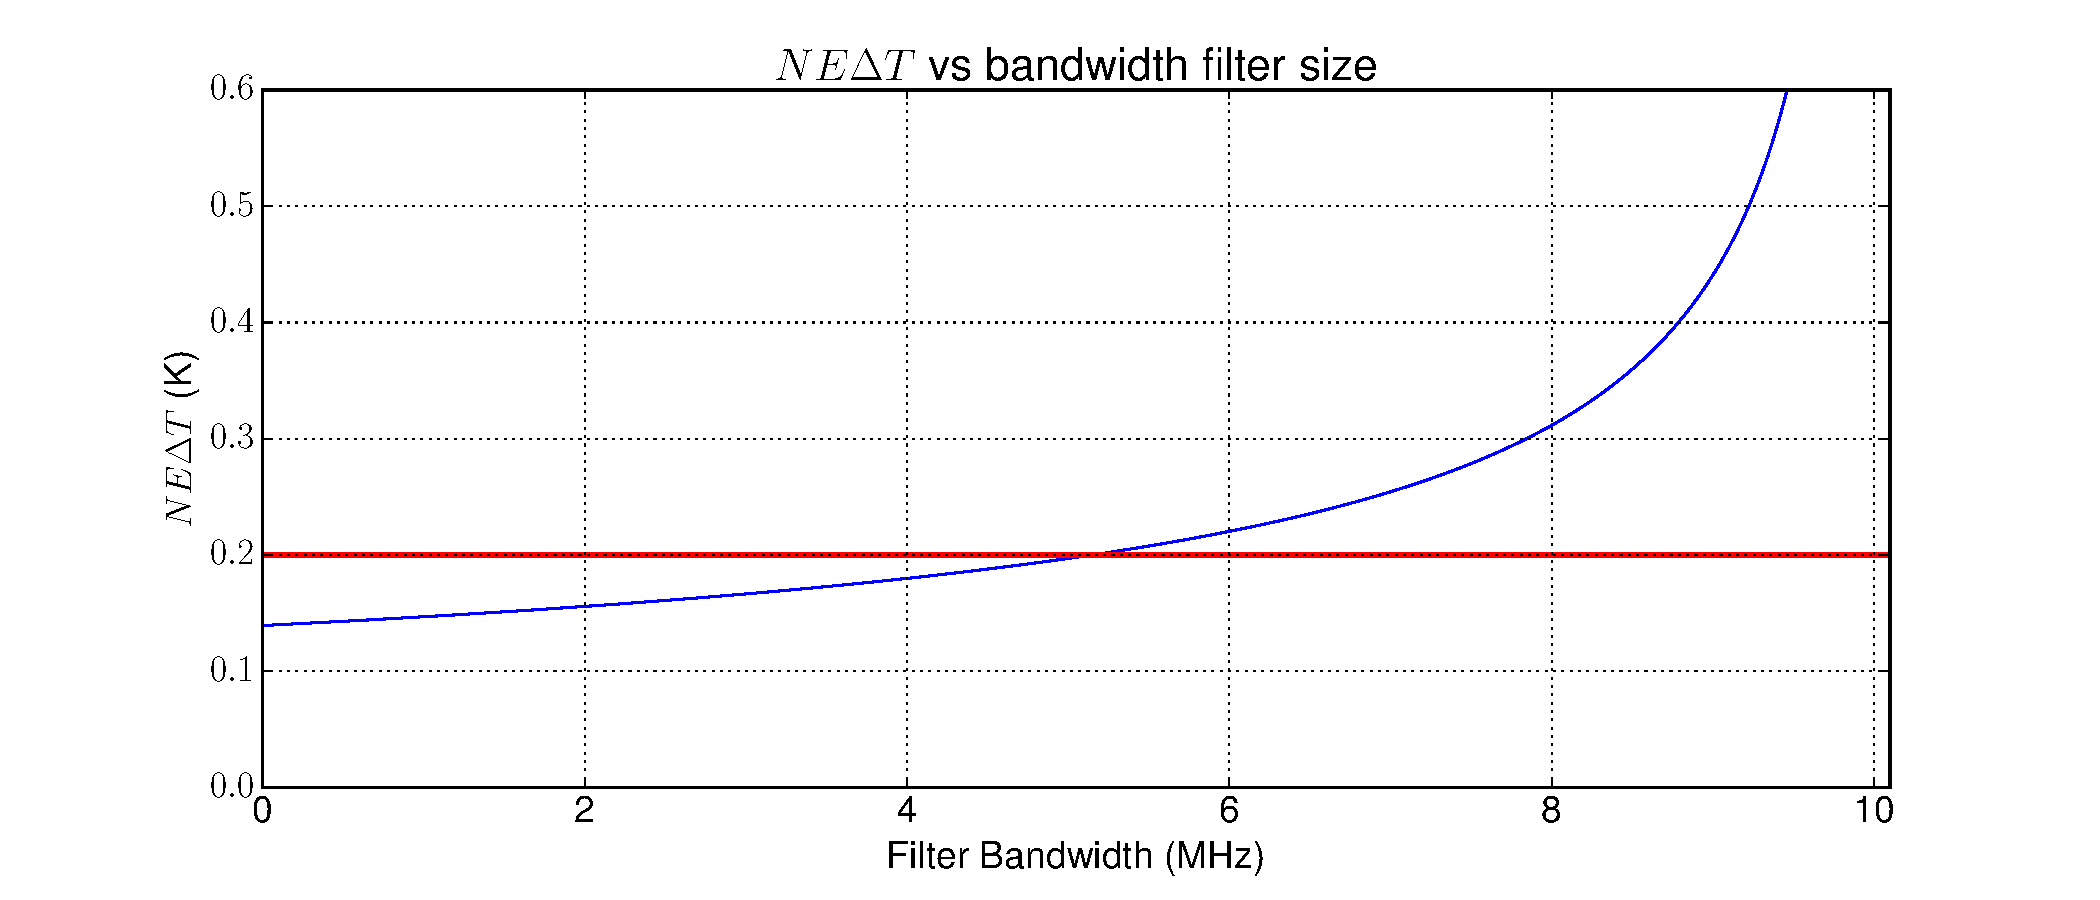
\includegraphics[width=\textwidth]{Experiments/Exp5/neatvsbw_plot.pdf}

\isucaption{Graph showing the impact of the filter to the $NE\Delta T$ performance of the radiometer}
\label{neatvsbw}
\end{figure}

Another impact that the filter has is how much power we expect to see at the radiometer.  We will refer to equation \ref{final_power} that shows the power received as a function of the bandwidth, gain, system noise temperature and measured noise temperature.  This equation is now re-written in \ref{eq:power_filter} to show that the bandwidth decreases as our filter bandwidth increases.

\begin{equation} \label{eq:power_filter}
P=k*(\beta - \beta_{filter})*G*(T_{A}+T_{N})
\end{equation}

A simple test was conducted that looked at what the theoretical power measured based on equation \ref{eq:power_filter} and what was measured with our SDR radiometer configuration.  Figure \ref{powervsbw} shows the results of this test.

\begin{figure}[h!tb] \centering

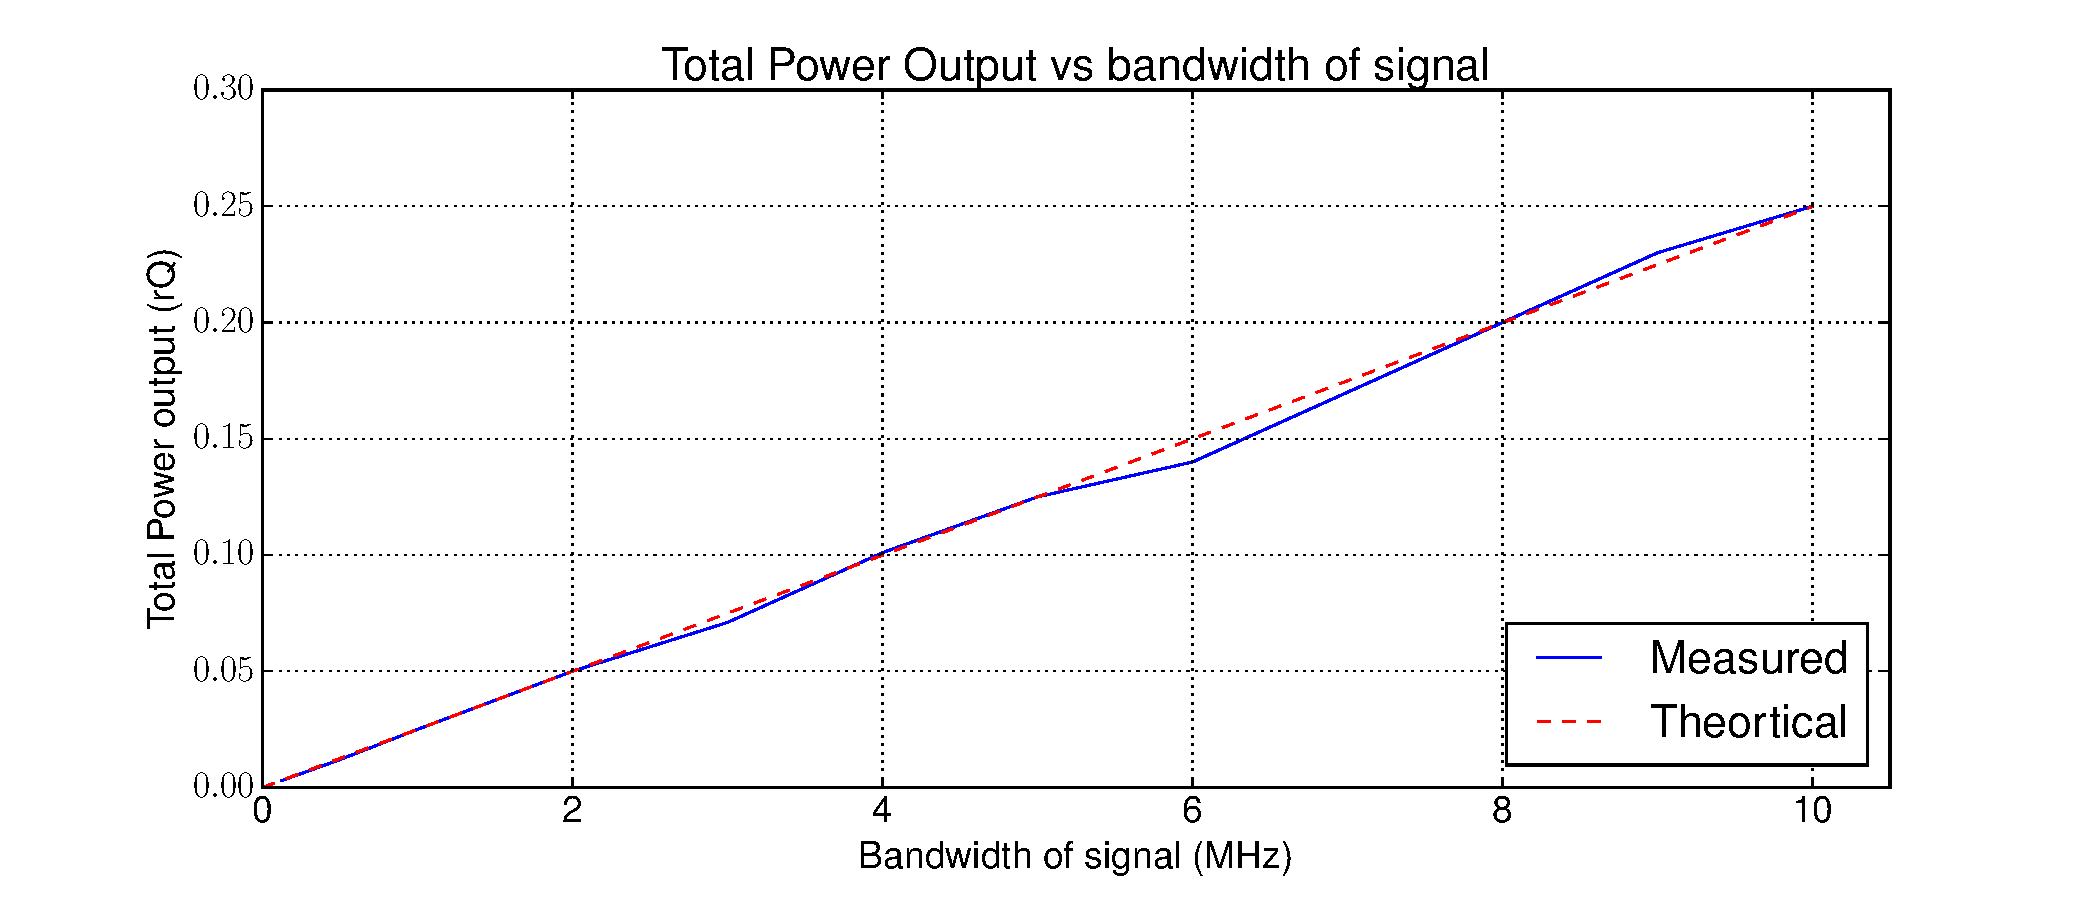
\includegraphics[width=\textwidth]{Experiments/Exp5/combined_plot.pdf}

\isucaption{Graph showing both theoretical and experimental data on the impact to the total power as a function of the bandwidth of the filter}
\label{powervsbw}
\end{figure}

As expected as the system increases the bandwidth of the filter, the total bandwidth seen is decreased and this results in a decrease in the total power that we might expect at the radiometer.  This means that at a certain point we may not be able to obtain the power information we need.

Filtering has other impacts to the signal that needs to be addressed.  Filtering a signal does have a cost associated with it in terms of the computational cost.  This depends on how tightly we need to have the filter and the sampling rate at which we are running the software defined radio.  In an ideal world we would have filters that have very steep frequency response rates.  However, this is computationally very expensive and so we often compromise by having less steep frequency response due to computational limits.  

Another factor with filters that does not directly impact the system but does need to be discussed is delays.  In the experiments in this thesis the graphs were compensated for delays due to the filters used.  A FIR filter that is used to filter out the offending signal has a very predictable delay and is computed in equations.  Another type of filter that is used is the IIR filter used in the power detection stage of the total power radiometer software.  An IIR filter however does not have a linear delay time and is instead based on the filter and the frequency it is filtering.  There are tools however that can be used to calculate this delay and this allows for us to properly compensate any delay with filtered signal.  This is important for doing comparison graphs with the square-law detector which does not use as many filters and does so at different frequencies.  

\subsection{Test Results}
We begin by looking at the what happens to our total power readings with no filter applied.  As we stated in the Lab Setup portion, the frequency of the offending signal will not change, but the amplitude will.  This will mean that we should see clear indications of the total power changing as the amplitude of the offending signal changes.  

\begin{figure}[h!tb] \centering

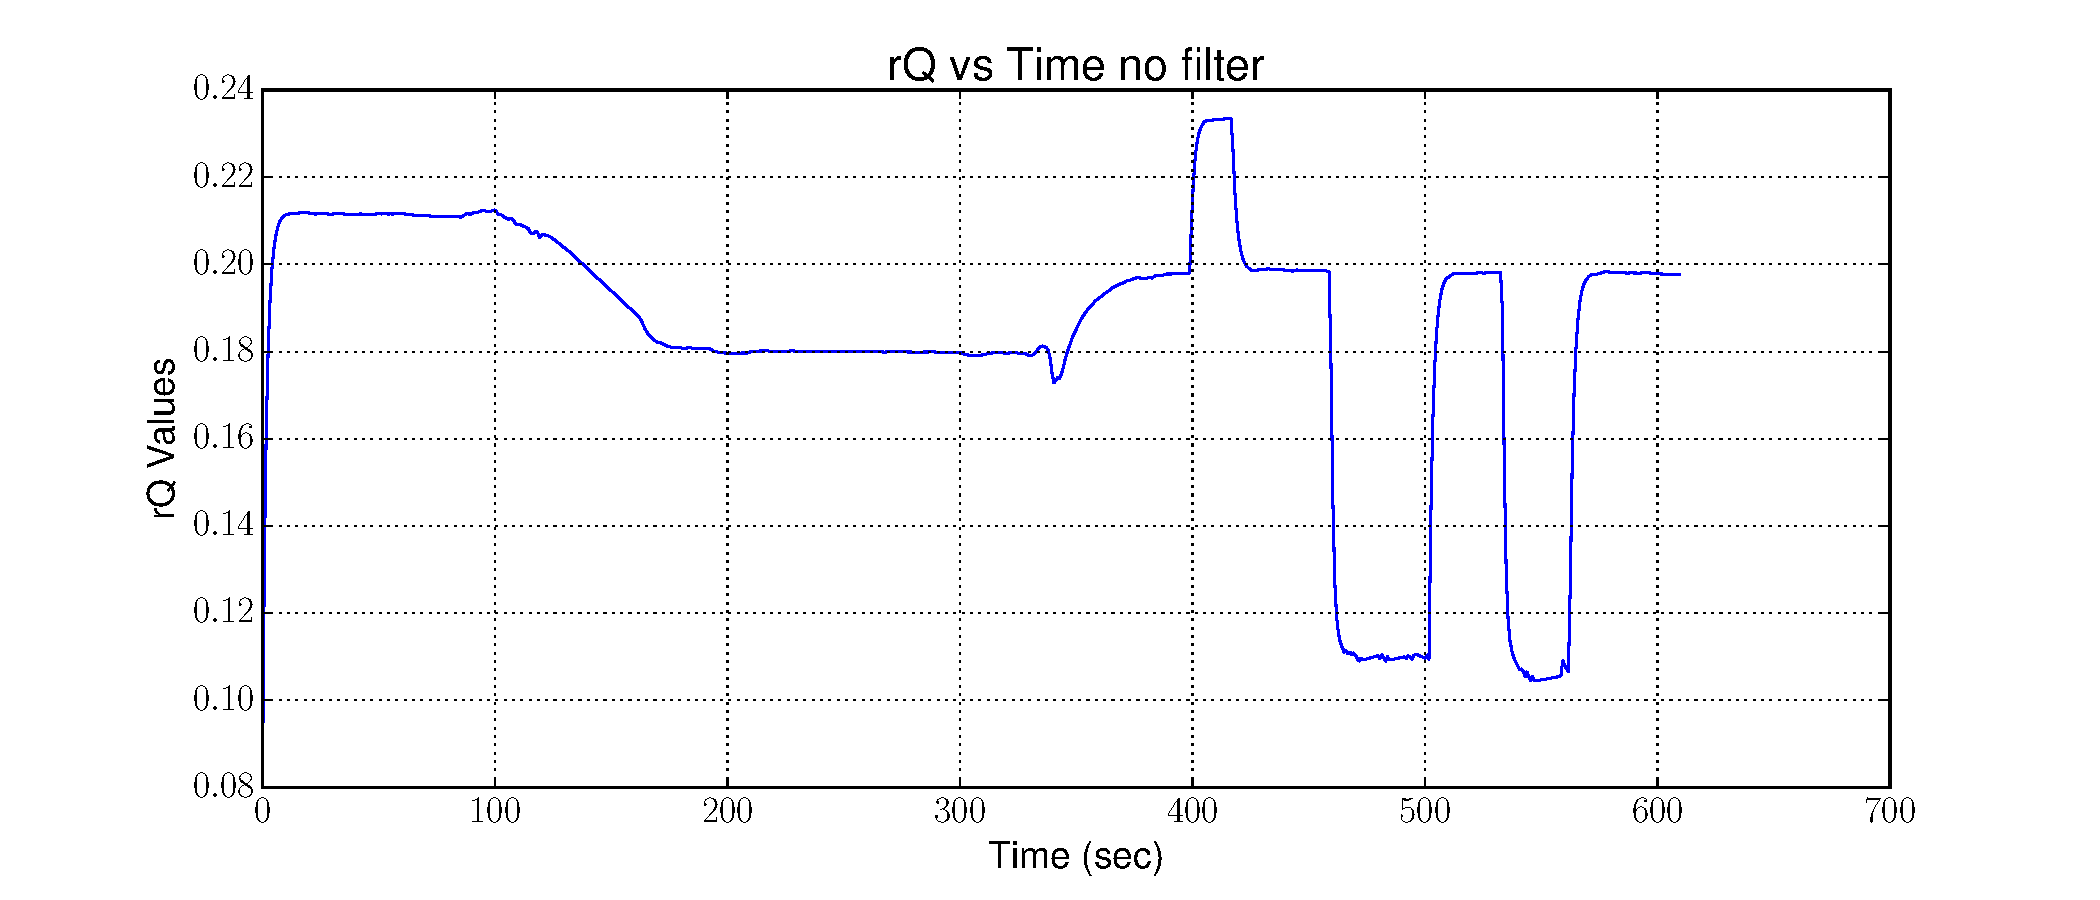
\includegraphics[width=\textwidth]{Experiments/Exp4/sdr_raw_unfiltered.pdf}

\isucaption{Graph showing the unfiltered total power measurements on the software defined radio}
\label{sdr_unfilt_raw}
\end{figure}

We can see that there are pulses that occur in the graph in figure \ref{sdr_unfilt_raw} and that changes in the amplitude of the offending signal affect our total power readings.  These same pulses can also be seen in the square-law detector data as well which can be seen in figure \ref{x2_unfilt}.

\begin{figure}[h!tb] \centering

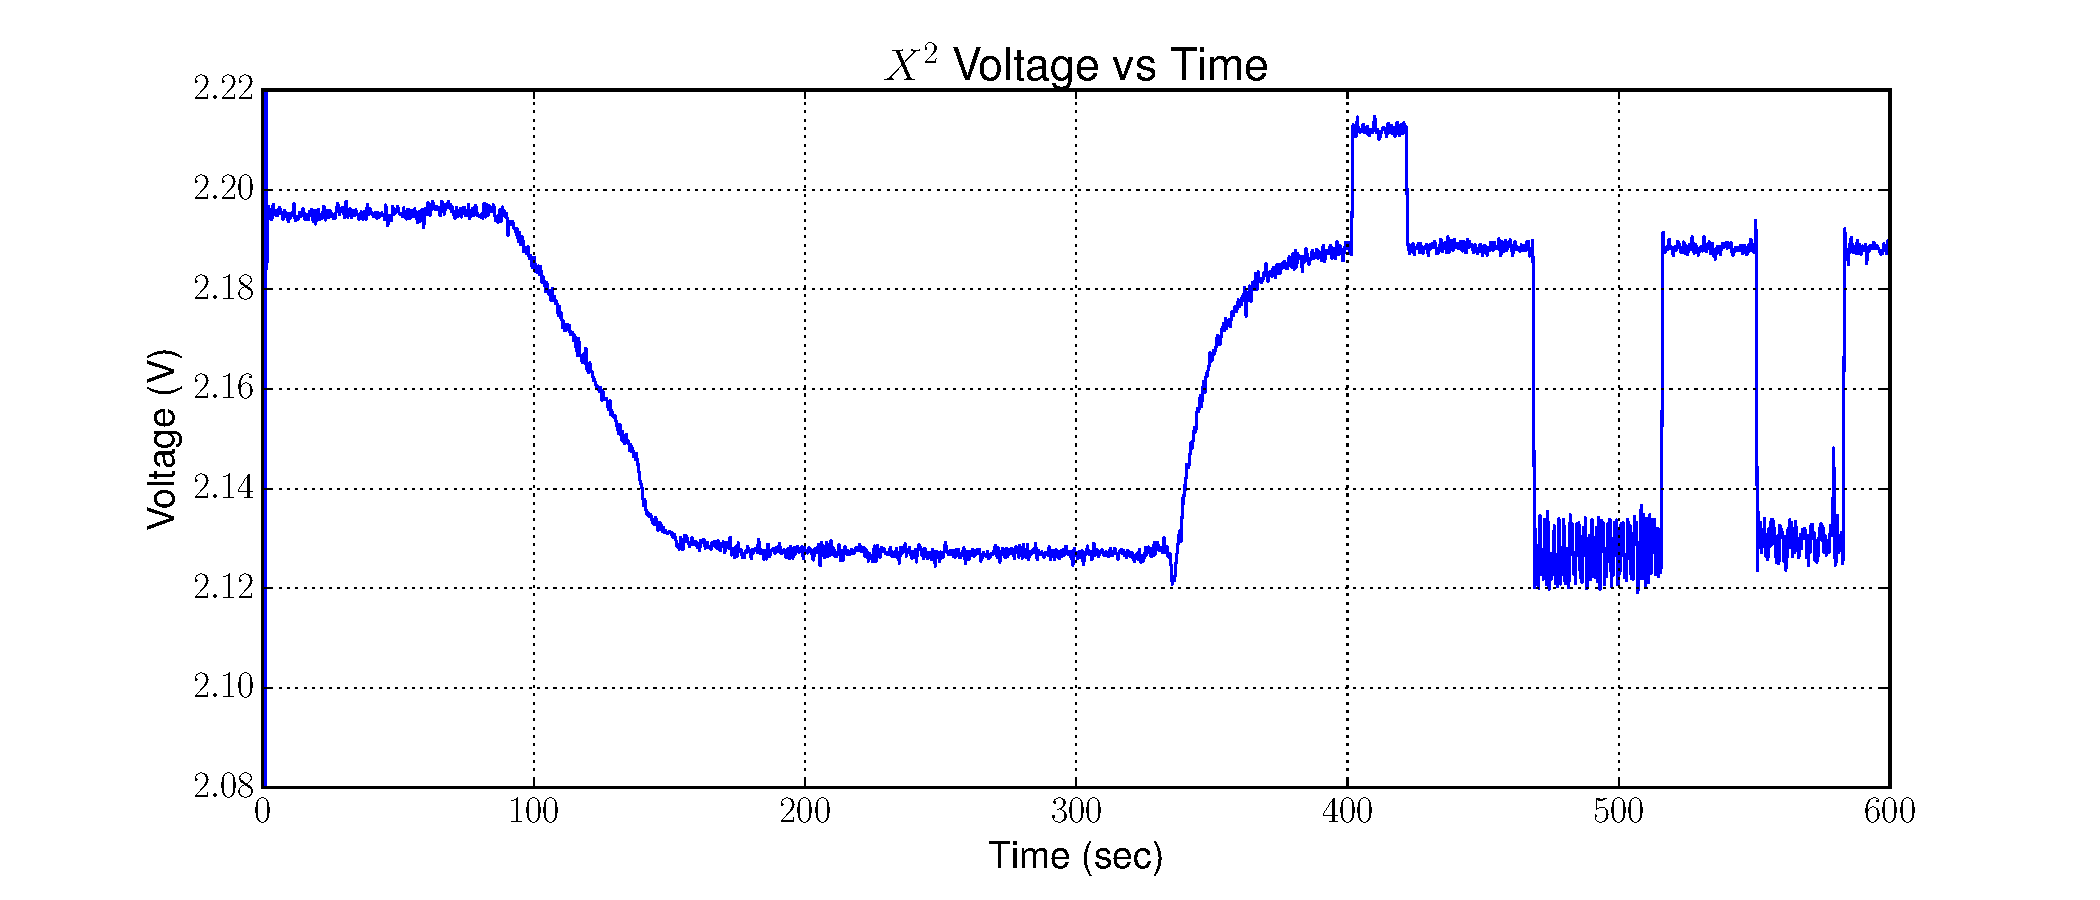
\includegraphics[width=\textwidth]{Experiments/Exp4/x2_voltage.pdf}

\isucaption{Graph showing the raw total power read from the square-law detector with an interfering signal.}
\label{x2_unfilt}
\end{figure}

We can clearly see in both the software defined radio and the square-law detector that there is an interfering signal.  If we now look at the spectrum view on the software defined radio, we can see the signal in questions which is at 1.405 GHz.  Figure \ref{spectrum_interfering} shows us what the software defined radio sees which is a spike at 1.405 GHz.  The square-law detector of course has no frequency information, so our only method to detect an interfering signal is by looking at the total power readings.  In our case there is elevated readings and we can see the spikes in the square-law data.  However, we do not know where in the spectrum the signal is at.

\begin{figure}[h!tb] \centering

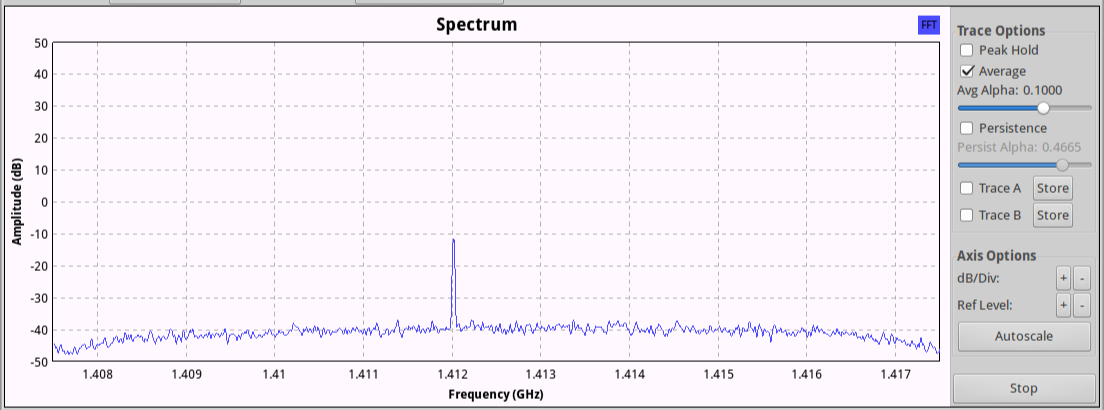
\includegraphics[width=\textwidth]{Images/spectrum_interference.png}

\isucaption{Image showing the spectrum view from the software defined radio}
\label{spectrum_interfering}
\end{figure}

Since we know where the offending signal is, we can now design our filter to filter out this signal.  In our GNURadio program we can specify both the frequency and the bandwidth our band-reject filter that we desire.  Ideally we want to keep the bandwidth of the filter as tight as possible to the offending signal but we also want to make sure our filter is effective in removing the signal.  Figure \ref{spectrum_filter} shows the spectrum display from the software defined radio with the filter now turned on and filtering the offending signal.

\begin{figure}[h!tb] \centering

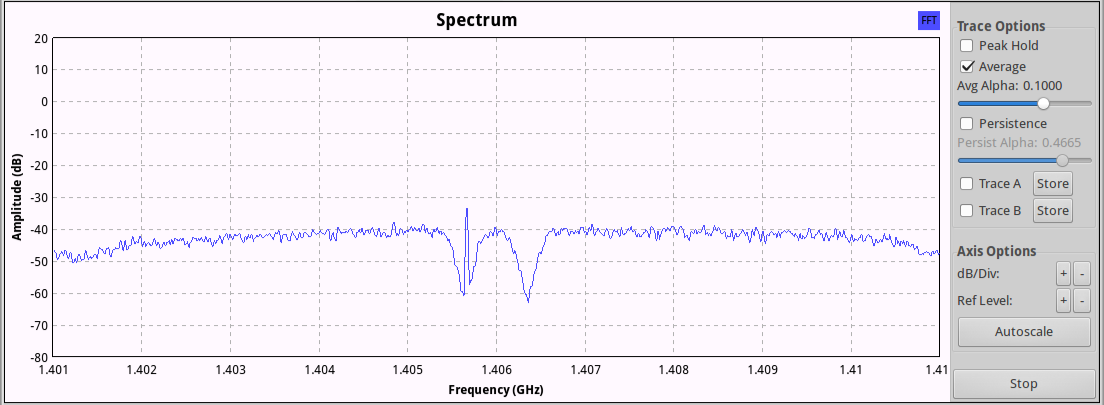
\includegraphics[width=\textwidth]{Images/spectrum_filter.png}

\isucaption{Image showing the software defined radio with the filter on and filtering the offending signal}
\label{spectrum_filter}
\end{figure}

Since we have now removed the offending signal, we will want to re-run our experiment and once again compare the difference between the software defined radio and the square law detector. We can begin by looking at the software defined radio total power readings.  In figure \ref{sdr_calib_filter} we can see a calibrated graph of the noise temperature seen by the software defined radio.  This graph is very similar to the graphs we expect from our total power radiometer.  However, we want to compare this to our square-law detector as well.  

\begin{figure}[h!tb] \centering

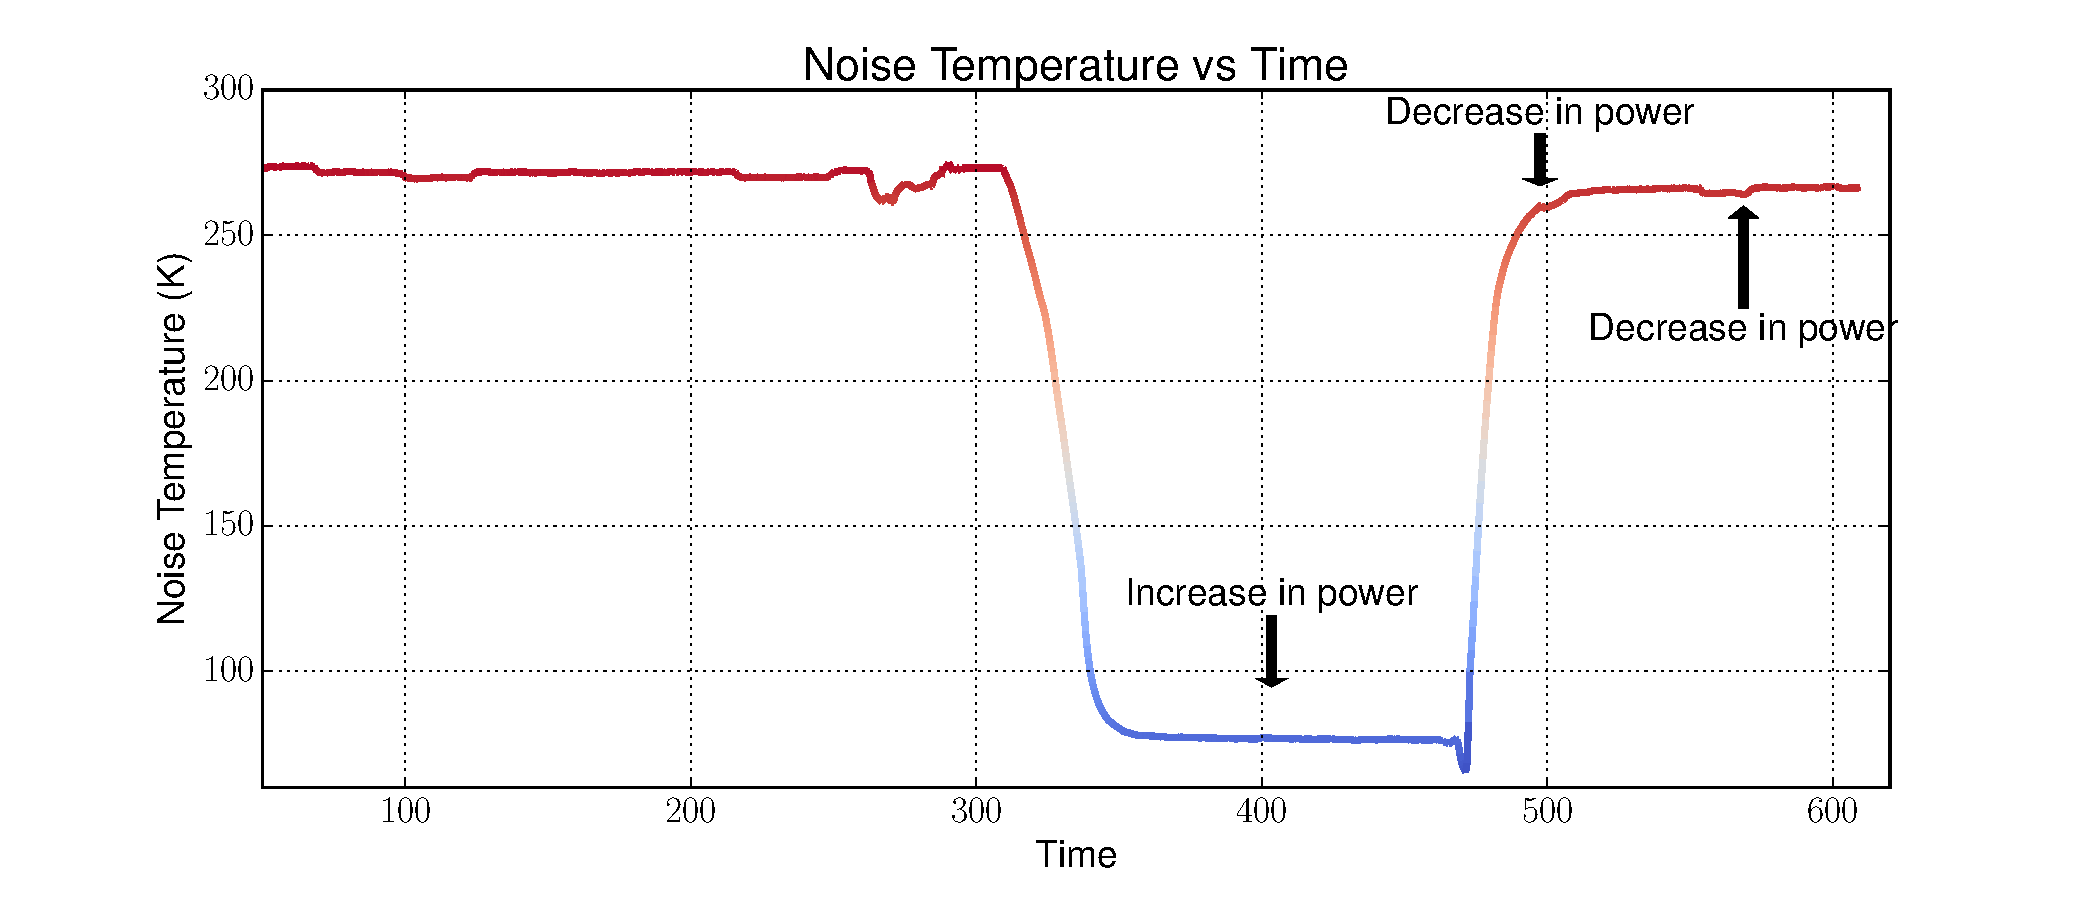
\includegraphics[width=\textwidth]{Experiments/Exp4/calib_filtered.pdf}

\isucaption{Graph showing the calibrated total power readings with the filter removing the offending signal}
\label{sdr_calib_filter}
\end{figure}

Figure \ref{filter_on} now shows both the software defined radio and the square-law detector calibrated total power readings.  In this graph you can see that the software defined radio is able to make normal readings where the square-law detector still shows the changes in amplitude which would make both calibration and obtaining useful data difficult.

\begin{figure}[h!tb] \centering

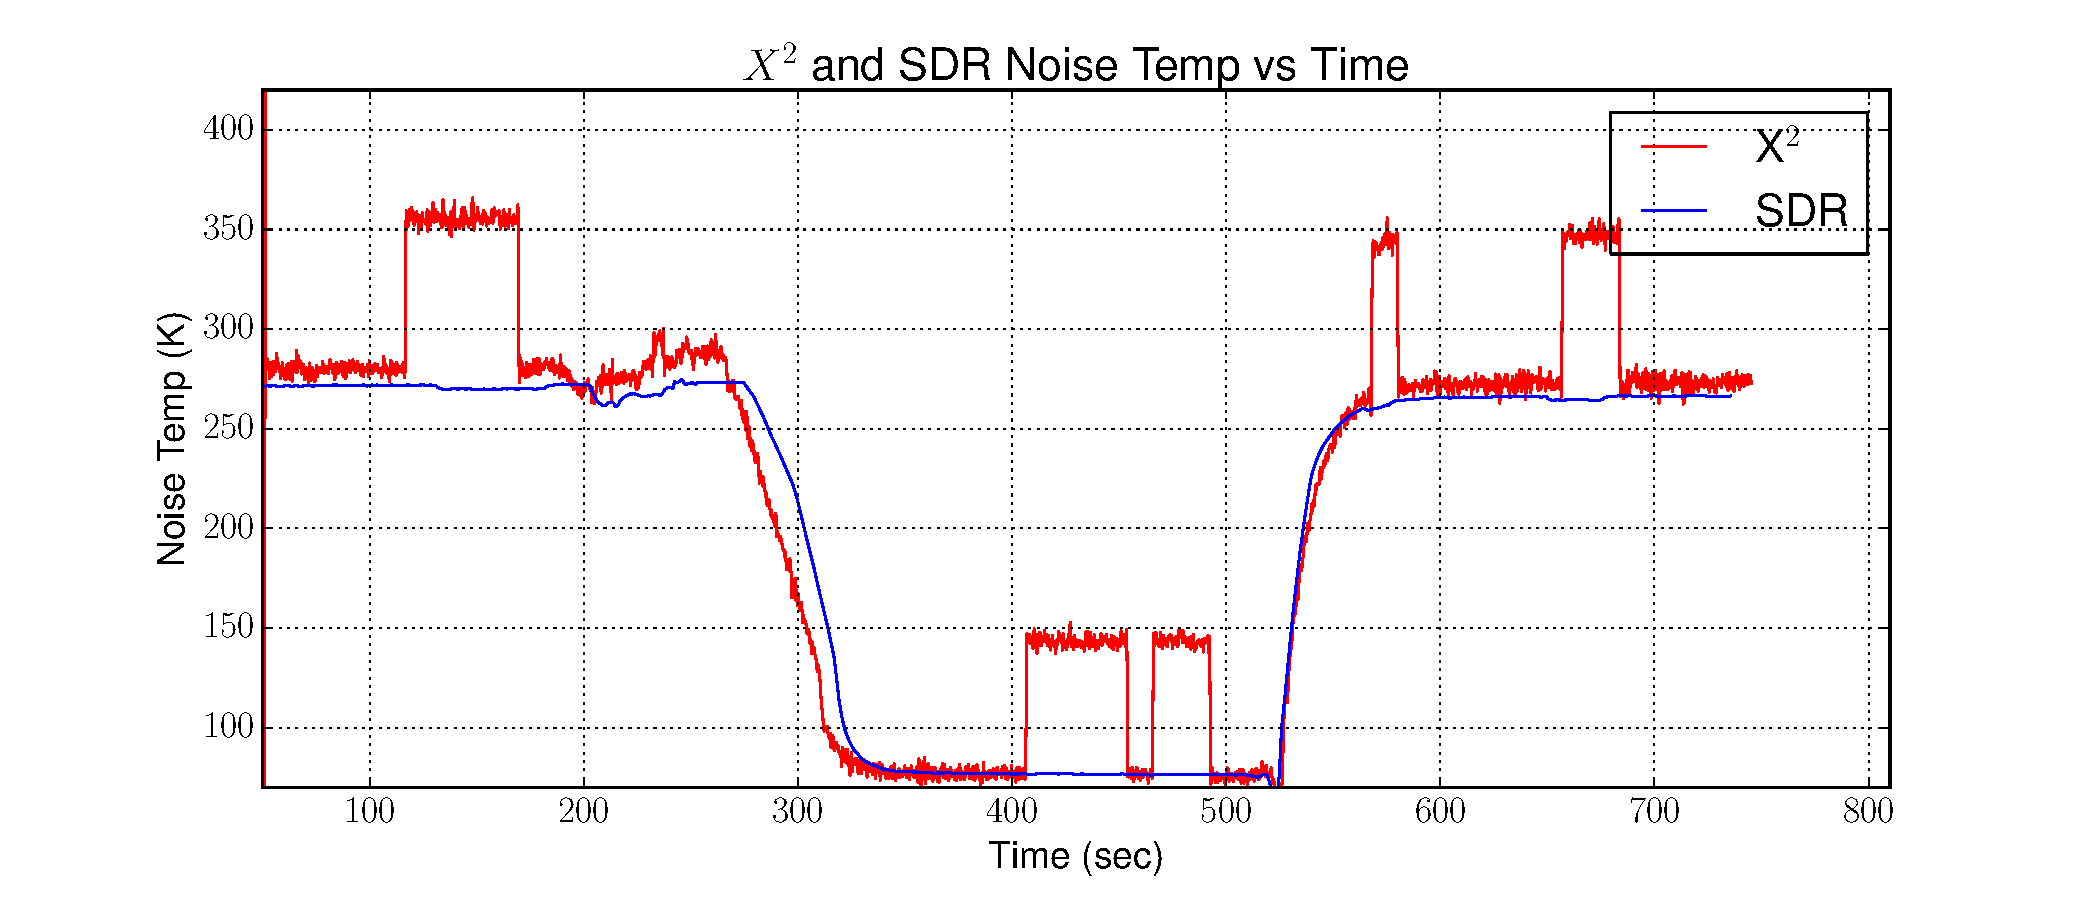
\includegraphics[width=\textwidth]{Experiments/Exp4/calib_filtered_both.pdf}

\isucaption{Image of the offending signal being filtered out by the SDR.  It can be seen that the signal is no longer visible.}
\label{filter_on}
\end{figure}

%----------------------------------------------------------
% End of Chapter 5.  Anything below this is extra information

%To verify the results of the information that the software defined radio is obtaining a square-law detector is used to measure the power of the incoming signal in parallel to the software defined radio.  This signal is split using a power divider so that the information will be the same to both devices with the except for the 3 dB plus insertion loss the power divider adds.  This allows us to verify the software defined radio with a proven system. 

%To test the ADL5902 a signal generator was used that had a controlled output.  The specific signal generator that was used was an older model that allowed us to change the output in 10 dBm increments.  The signal generator was also configured for 1.4 GHz as that is the frequency the ISU RF front end is configured to listen at.  Ideally a noise generator would have been desirable, however a noise generator with adjustable power output could not be located on campus.  

%The ADL5902 is available from Analog Devices in an evaluation board.  This board pairs the ADL5902 with a AD7466 12-bit analog to an analog to digital converter.  This board can then be mated with Analog Devices BlackFin processor which acts as a USB gateway for the AD7466 data.  A test program written in LabView is also provided as well.

%The test program provided by Analog Devices allows us to query the ADL5902 and record the raw ADC value.  This program also allows us to enter in the frequency used during testing, the temperature during the test, and allowed for calibration of the ADL5902.  All of the data is then stored into an Excel spreadsheet which can be accessed later.

%For this test we used the signal generator set to 1.4 GHz and started at $-60$ dBm for the output signal.  This was selected as this is the lowest the square law detector can detect.  The output power was then incremented on the signal generator in 10 dBm steps.  There was no change to any other parameter.  This was done up to 0 dBm.  Any higher and there was risk of damage to the ADL5902.  This test was then repeated several times and was done with the signal generator stepping up from $-60$ dBm to 0 dBm and from 0 dBm to $-60$ dBm.  

%The square-law detector that we obtained is the Analog Devices ADL5902.  The ADL5902 is a true rms responding power detector that has a square law detector, a variable gain amplifier, and an output driver. It also has a temperature sensor and will compensate for temperature variations.  The output driver allows for the small signal from the square law detector to be amplified to a level that most analog to digital devices can detect.  It should be noted that this is not an amplifier for the incoming RF signal, just to amplify the small signal from the diode.  This driver however does have low noise and has a noise output of approximately $25nV/ \sqrt{Hz}$ at 100 kHz.  The ADL5902 operates from 50 MHz to 9 GHz and in most cases can detect down to $-60$ dBm.  This works well in our application since the radiometer operates at 1.4 GHz and after the amplification stage we usually see between $-40$ to $-30$ dBm of power.  

%{\begin{figure}[h!tb] \centering
%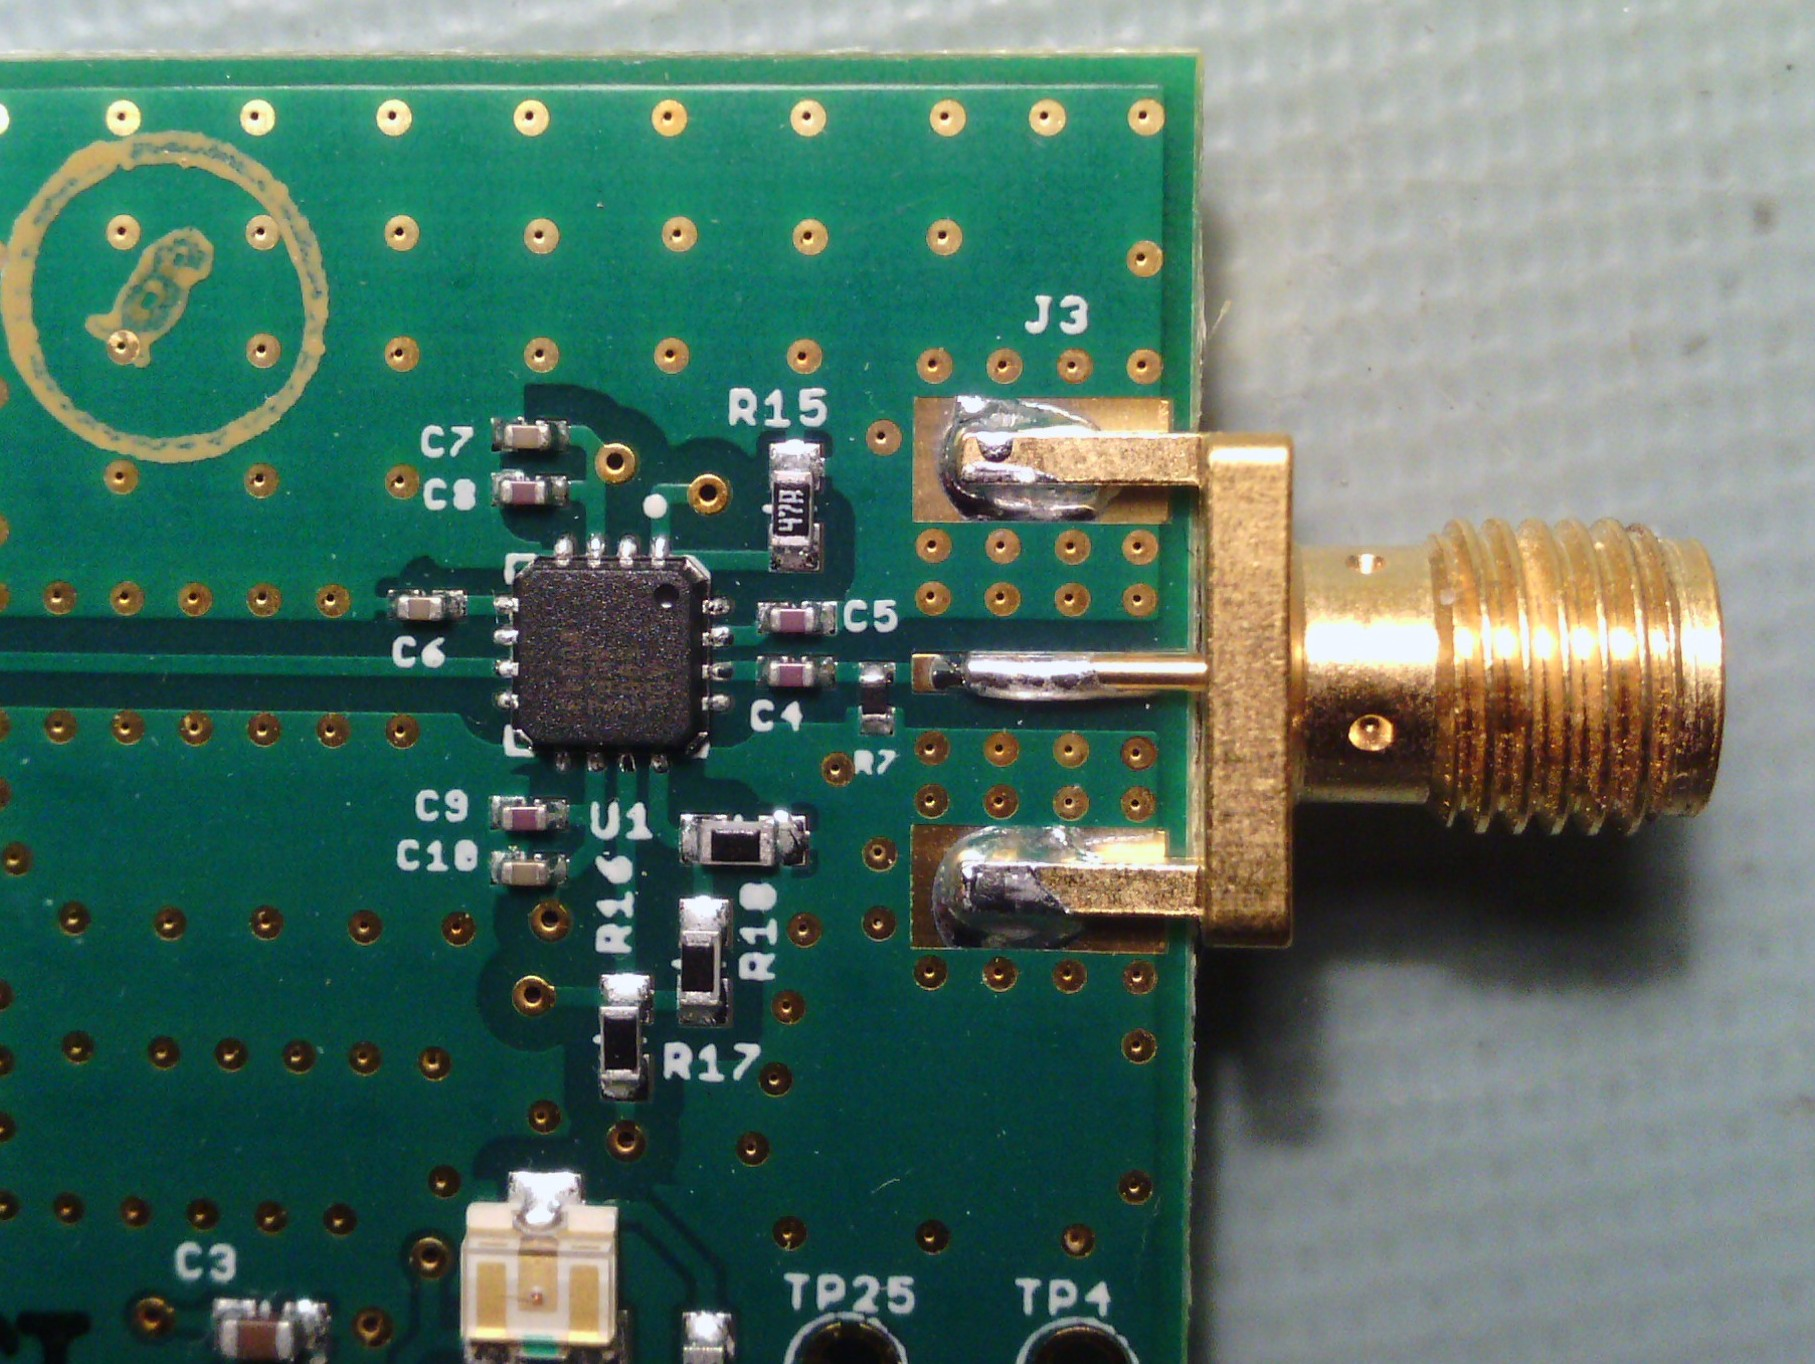
\includegraphics[width=\textwidth]{Images/adl5902.jpg}
%\isucaption{An image of the ADL5902 square-law detector used in these experiments}
%\label{ADL5902}
%\end{figure}
%}

%The specifications of the ADL5902 can be seen in Table~\ref{ADL5902_data} shown below.

%\begin{table}[h!tb] \centering
%\isucaption{ADL5902 Specifications}
%\label{ADL5902_data}
%\begin{tabular}{lcc} \hline
%\textbf{Parameter @ 900 MHz} & \textbf{Value} & \textbf{Units} \\ \hline
%Frequency Range & 50 to 9000 & MHz \\
%Dynamic Range & 61 & dB \\
%Minimum Input Level, $\pm 1.0$ dB & 60 & dB \\ 
%Maximum Input Level, $\pm 1.0$ dB & 1 & db \\
%Logarithmic Slope & 53.7 & mV/dB \\ 
%Output Voltage Range & 0.03 to 4.8 & V \\ \hline
%\end{tabular}
%\end{table}

%The ADL5902 outputs an analog signal that falls between 0.03 volts and 4.8 volts.  It outputs a change of 53.7 millivolt per dB detected by the ADL5902. 